\documentclass[12pt]{article}
%Gummi|065|=)
\usepackage{amsmath, amsfonts, amssymb}
\usepackage[margin=0.5in]{geometry}
\usepackage{xcolor}
\usepackage{graphicx}

\newcommand{\off}[1]{}
\DeclareMathSizes{20}{30}{20}{18}

\newcommand{\two }{\sqrt[3]{2}}
\newcommand{\four}{\sqrt[3]{4}}


\usepackage{tikz}

\title{Item: \textbf{Cohomology of Arithmetic Groups}}
\author{John D Mangual}
\date{}
\begin{document}

\fontfamily{qag}\selectfont \fontsize{12.5}{15}\selectfont

\maketitle

\noindent The Eichler-Shimura isomorphism let's you express weight-2 modular forms theory into cohology of $\text{SL}_2(\mathbb{Z})$. This will take a lot of effort to unpack.  One version I have found says these two are the same:
\begin{itemize}
\item $f(z) \, dz$ is a $\Gamma$-invariant form on $\mathbb{H}$
\item $[ \, f(z) dz \, ] \in H^1 (\mathbb{H}/\Gamma, \mathbb{C}) = H^1(\Gamma, \mathbb{C})$
\end{itemize}
but these are two different kinds of cohomology.  One of them is a hyperbolic space $\mathbb{H}/\Gamma$ and the other is a group of $2 \times 2$ matrices $\Gamma \subseteq \text{SL}_2(\mathbb{Z})$.  How can we not have a complete understanding of both of these objects? \\ \\
There's a trade-off between generality and our ability to supply details.  I never told you what $\Gamma$ was, and the entire textbook writes the discussion without naming a specific answer.  How can they have the best possible answer?  If, I decide to focus on one $\Gamma$, let's say $\Gamma_0(4) = \langle z \mapsto z + 1, z \mapsto - \frac{1}{4z}\rangle$ maybe I will say things that don't generalize.  \\ \\
In between, would be story where I examine many possible $\Gamma$ and a statement will be true in cases and not others (in many cases and not others). I might even be able to express this type of meta-logic using a small amount of category theory. \\ \\
Let's find a modular form of weight 2.  The first one I can think of is a theta-function raised to the 4th power:
$$  \theta(z) = \big( \sum q^{n^2} \big)^4 = \sum r_4(n) \, q^n $$
and here $\Gamma_0(4) \neq \text{SL}_2(\mathbb{Z})$. How do we know it is modular form of weight 2?  This is a great example if we keep in mind the following recipe:
$$ \text{M}_2(\Gamma_0(N)) = \text{S}_2(\Gamma_0(N)) \oplus \text{E}_2(\Gamma_0(N)) $$
for all congruence groups, not just $N = 4$.  This says every weight two modular form splits into to parts:
\begin{itemize}
\item Eisenstein series
\item Cusp forms ( Poincar\'{e} series )
\end{itemize}
The jargon gets worse and worse.  Eichler-Shimura theory, Atkin-Lehmer theory.   If I have an interestng number theory problem, maybe I can turn it into a modular forms problem:
$$ \text{modular forms} \stackrel{?}{\not =} \text{number theory} $$
I cannot find any modular forms of weight 2 that are not Eisenstein series until $\Gamma_0(11)$

\newpage

\noindent The formula I found on the internet is a \textbf{newform}\footnote{\texttt{http://www.lmfdb.org/ModularForm/GL2/Q/holomorphic/11/2/1/a/}} and the coefficient field is $\mathbb{Q}$ (in fact they're in $\mathbb{Z}$) and we get the first fiew terms and Satake parameters (which sound useful). 
$$ \eta(z)^2 \eta(11z)^2 = q \prod_{n=1}^\infty (1-q^n)^2 (1 - q^{11n})^2  = q - 2q^2 - q^3 + 2q^4 + q^5 + 2 q^6 - 2 q^7 - 2q^9 + \text{O}(q^{10})$$
It is not obvious to me these coefficients are multiplicative (except $a_{11} = +1$), in that case:
$$ a_2 \times a_3 = (-2) \times (-1) = + 2 = a_6 $$
The coefficients don't seem to match up since perfect powers they are not multiplicative:
$$ a_2 \times a_2 \times a_2 = (-2)\times (-2)\times (-2) = -8 \neq 0 = a_8 $$
The L-function is found by moving the q-series $q^n$ to Dirichlet-series $n^s$ as done by the \textbf{Mellin transform}
$$ L(f,s) = 1^s -2 \times 2^s - 1 \times 3^s + 2 \times 4^s + 1 \times 5^s + 2 \times 6^s  + \dots = \left( 1 - \frac{a_{11}}{11^s} \right)^{-1} \prod_{p \neq 11} \left( 1 - \frac{a_p}{p^s} \right)^{-1} $$
Eichler-Shimura maps the newforms (or Eisenseries) over this group and maps them to elements of group cohomology
$$ \int_0^{11} \eta(z)^2 \eta(11z)^2 \; dz = \text{???} $$
and now for a homework question: what are the other cycles of $\Gamma_0(11)$ ? Not so easy.\footnote{\texttt{http://wstein.org/books/modform/modform/modform.html}}
$$ \Gamma_0(N) = \left\{ \left( \begin{array}{cc} a & b \\ c & d \end{array}   \right) \in \text{SL}_2(\mathbb{Z}) : 
\left( \begin{array}{cc} a & b \\ c & d \end{array}   \right)  \equiv
\left( \begin{array}{cc} \ast & \ast \\ 0 &  \ast  \end{array}  \right) \pmod{ N }
 \right\} $$
 Where is also $\Gamma_1(N)$ with a more strict equivalence relation.   The equation $ad-bc=1$ says they are neighbors on the Farey fraction list:
 $$ \dots  < \frac{a}{c} <  \frac{b}{d} < \dots $$
so the cosets $[\text{SL}_2(\mathbb{Z}) : \Gamma_0(N)]$ is indexed by the Farey fractions $\pmod {N}$ (I just took that from a textbook) so there should be \textbf{11+1=12} cosets.  Neither of these is normal subgroup with exact sequence:
$$ 1 \to \Gamma(N) \to \text{SL}_2(\mathbb{Z}) \to \text{SL}_2( \mathbb{Z}/N\mathbb{Z}) \to 1 $$
We will have time to test my intuition for algebra later (as is already happening!). \\

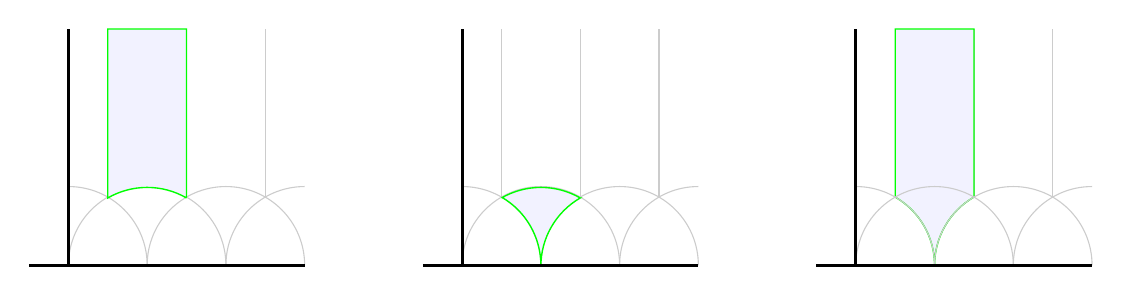
\begin{tikzpicture}

\draw[color=black!20!white] (0.5, 3)--(0.5, 0.866);
\draw[color=black!20!white] (1.5, 3)--(1.5, 0.866);
\draw[color=black!20!white] (2.5, 3)--(2.5, 0.866);


\draw[color=black!20!white] (3,0) arc (0  :180:1);
\draw[color=black!20!white] (2,0) arc (0  :180:1);
\draw[color=black!20!white] (1,0) arc (0  : 90:1);
\draw[color=black!20!white] (2,0) arc (180: 90:1);

\draw[fill=blue!5!white, line width=0.5, draw=green] 
(1.5,0.866)--(1.5,3)--(0.5,3)--(0.5,0.866)--
(0.5, 0.855) arc (-60:-120:-1);

\draw[line width = 1] (-0.5,0)--(3,0);
\draw[line width = 1] (0,3)--(0,0);

\begin{scope}[xshift=5cm]

\draw[color=black!20!white] (0.5, 3)--(0.5, 0.866);
\draw[color=black!20!white] (1.5, 3)--(1.5, 0.866);
\draw[color=black!20!white] (2.5, 3)--(2.5, 0.866);


\draw[color=black!20!white] (3,0) arc (0  :180:1);
\draw[color=black!20!white] (2,0) arc (0  :180:1);
\draw[color=black!20!white] (1,0) arc (0  : 90:1);
\draw[color=black!20!white] (2,0) arc (180: 90:1);

\draw[fill=blue!5!white, line width=0.5, draw=green] 
(0.5, 0.855) arc (-60:-120:-1)--
(1.5, 0.855) arc (-60:0:-1)--
(1,0) arc (0:60:1);

\draw[line width = 1] (-0.5,0)--(3,0);
\draw[line width = 1] (0,3)--(0,0);

\end{scope}

\begin{scope}[xshift=10cm]


\draw[color=black!20!white] (0.5, 3)--(0.5, 0.866);
\draw[color=black!20!white] (1.5, 3)--(1.5, 0.866);
\draw[color=black!20!white] (2.5, 3)--(2.5, 0.866);


\draw[fill=blue!5!white, line width=0.5, draw=green] 
(0.5,0.866)--(0.5,3)--(1.5,3)--(1.5,0.866)--
(1.5, 0.866) arc (-60:0:-1)--
(1,0) arc (0:60:1);

\draw[color=black!20!white] (3,0) arc (0  :180:1);
\draw[color=black!20!white] (2,0) arc (0  :180:1);
\draw[color=black!20!white] (1,0) arc (0  : 90:1);
\draw[color=black!20!white] (2,0) arc (180: 90:1);




\draw[line width = 1] (-0.5,0)--(3,0);
\draw[line width = 1] (0,3)--(0,0);

\end{scope}

\end{tikzpicture}

\newpage

\noindent The question at hand is why there is a weight 2 modular form at ``level" 11.  These terms level and weight are the most ambiguous terms I have ever used.  Here is some of the table from LMFDB: \\

\begin{tabular}{r|rrrrrrrrrrrrrrrr}

 \textbf{level} & 1 & 2 & 3 & 4 & 5 & 6 & 7 & 8 & 9 & 10 & 11 & 12 & 13 & 14 & 15 \\ \hline
\textbf{weight }2 & 0 & 0 & 0 & 0 & 0 & 0 & 0 & 0 & 0 & 0  & \color{red!60!white}{\textbf{1}}  & 0  & 0  &  1 &  1 \\ 
4 & 0 & 0 & 0 & 0 & 1 & 1 & 1 & 1 & 1 & 1 & 2  & 1  & 3  & 2  &  2 
\end{tabular} \\ \\
These modular forms are the raw materials.  Fustratingly, I took for granted the connection between modular forms and number theory.  The connections between number theory and geometry get packaged away into theorems, preventing real insight from occuring. \\ \\
These tables are not enough for me.  \\ \\
The program was: learn modular forms, solve problems in number theory.  It still hasn't happened.  Something about the way textbooks are written. \\ \\
My best guess is that $11 + 1 = 3 \times 4$ is just enough ``volume" for a weight 2 modular form to occur.  \\ \\ 
All modular forms break up into newforms and Eisenstein series and we are told there's no newforms before a certain point.  Hopefully I haven't mixed up ``newform" and ``cusp form".  \\ 

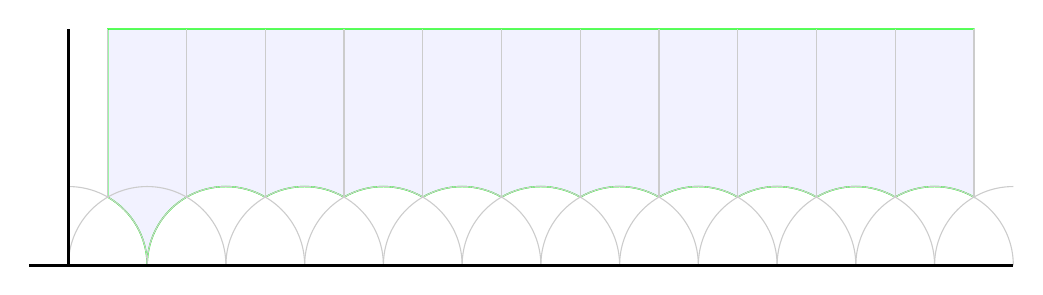
\begin{tikzpicture}

\draw[fill=blue!5!white, line width=0.5, draw=green] 
(0.5,0.866)--(0.5,3)--(11.5,3)--(11.5,0.866)--
(11.5, 0.866) arc (60:120:1)--
(10.5, 0.866) arc (60:120:1)--
( 9.5, 0.866) arc (60:120:1)--
( 8.5, 0.866) arc (60:120:1)--
( 7.5, 0.866) arc (60:120:1)--
( 6.5, 0.866) arc (60:120:1)--
( 5.5, 0.866) arc (60:120:1)--
( 4.5, 0.866) arc (60:120:1)--
( 3.5, 0.866) arc (60:120:1)--
( 2.5, 0.866) arc (60:120:1)--
( 1.5, 0.866) arc (-60:0:-1)--
( 1,0) arc (0:60:1);

\foreach \a in {0,...,11} {

	\draw[color=black!20!white] (0.5 + \a , 3)--(0.5 + \a , 0.866);

}



\foreach \a in {2,...,12} {
	\draw[color=black!20!white] ( \a ,0) arc (0  :180:1);
}


\draw[color=black!20!white] (1 ,0) arc (0  : 90:1);
\draw[color=black!20!white] (11,0) arc (180: 90:1);


\draw[line width = 1] (-0.5,0)--(12,0);
\draw[line width = 1] (   0,3)--( 0,0);


\end{tikzpicture}  \\ \\
This is a quick drawing.  The natural question: how does a circle cut these shapes? Since I have written: $ \eta(z)^2 \eta(11z)^2 $ is the weight-2 modular form let's check:
$$ \eta(z)^2 \, \eta(11z)^2 \, dz \text{ is invariant under } \Big\langle z \mapsto z + \frac{1}{11}, z \mapsto - \frac{1}{z} \Big\rangle $$
I don't see why multiplying four copies of the eta function doesn't already give weight 2 modular form.  Just by $4 \times \frac{1}{2} = 2$.  

\vfill

\fontfamily{qag}\selectfont \fontsize{12}{10}\selectfont

\begin{thebibliography}{}

\item John Cremona \textbf{The L-functions and modular forms database project}  \texttt{arXiv:1511.04289}  
\texttt{http://www.lmfdb.org/}

\item William Stein \textbf{Modular Forms, A Computational Approach} Modular forms of Weight 2 \texttt{http://wstein.org/books/modform/modform/index.html}

\item Christoph Schmitt. \textbf{Calculation of L-Functions Associated with
Newforms: Implementation, Choice of
Parameters and Verification of Zero} (Diplomarbeit, 2010)

\end{thebibliography}

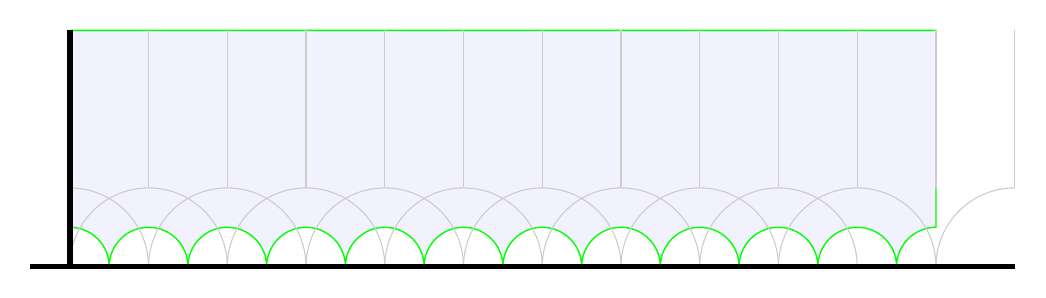
\begin{tikzpicture}

\draw[fill=blue!5!white, line width=0.5, draw=green] 
(0,0.5) arc (90:0:0.5)--
(0.5,0) arc (180:0:0.5)--
(1.5,0) arc (180:0:0.5)--
(2.5,0) arc (180:0:0.5)--
(3.5,0) arc (180:0:0.5)--
(4.5,0) arc (180:0:0.5)--
(5.5,0) arc (180:0:0.5)--
(6.5,0) arc (180:0:0.5)--
(7.5,0) arc (180:0:0.5)--
(8.5,0) arc (180:0:0.5)--
(9.5,0) arc (180:0:0.5)--
(10.5,0) arc (180:90:0.5)--
(11,0.5)--(11,3)--(0,3);

\foreach \a in {0,...,12}{

	\draw[color=black!20!white] (\a, 3)--(\a, 1);
	%\draw[color=black!20!white] (\a+0.5,0.5) arc (60:120:1);

}

\foreach \a in {2,...,11}{
	
	\draw[color=black!20!white] (\a ,0) arc (0:180:1);

}

\draw[color=black!20!white] (1,0) arc (0:90:1);
\draw[color=black!20!white] (11,0) arc (180:90:1);



\draw[line width = 2] (-0.5,0)--(12,0);
\draw[line width = 2] (0,3)--(0,0);


\end{tikzpicture}

\end{document}